\section{Workload Characterization}
\label{sec:workloadchar}

As a follow-up to our characterization of the Spider 1 storage system, below we
will be presenting a comparative analysis of the I/O workloads observed on the
Spider systems. Our analysis focuses on I/O usage trends and I/O request
characteristics.


\subsection{I/O Usage Trends}

\subsubsection{Read vs. Write Operations}


Figure~\ref{fig:rwratio} shows the read vs. write balance observed on the two
Spider systems.  As can be seen, there is a slight imbalance in the total write
requests for 50\% of the controllers sampled in the Spider 2 system. This
imbalance is because the upper level file systems are imbalanced. As we stated
above, we deployed two file system namespaces on  non-overlapping hardware
resources. The file systems are allocated across projects at the OLCF and some
projects have been heavier I/O consumers than others, and we have observed 
that some projects are transferring large datasets to the OLCF for processing 
on Titan. It turns out that the ``atlas1'' partition is being utilized at a 
higher rate.  In general we see a higher percentage of write operations on 
Spider 2 as compared to Spider 1. This meets our design expectations for 
handling large memory checkpoints with  minimal reading of those checkpoint 
data files. Also, it is quite visible in Figure~\ref{fig:rwratio}(b)
that ``atlas1'' portion of Spider 2 is 10\% more write-intensive than the
Atlas2 (left half vs. the right half of the Figure~\ref{fig:rwratio}(b). 
This discrepancy is due to the same factors and since being corrected the 
trend is moving back toward the expected balance. Finally, as can be seen 
in Figure~\ref{fig:rwratio}, approximately 60\% of the I/O workload on 
Spider 1 was write operations and 40\% was reads. Spider 1 was a center-wide 
resource shared across all OLCF platforms and the high percentage of the read 
requests was attributed to analysis and data transfer I/O workloads accessing 
Spider 1. Spider 2 is also a center-wide shared resource, but it has a higher 
percentage of write operations than Spider 1 (approximately 75\% vs. 
approximately 60\%), we have concluded that the way the system is being 
used accounts for the differences.  

\begin{figure}[!t]
\begin{center}
\begin{tabular}{c}
{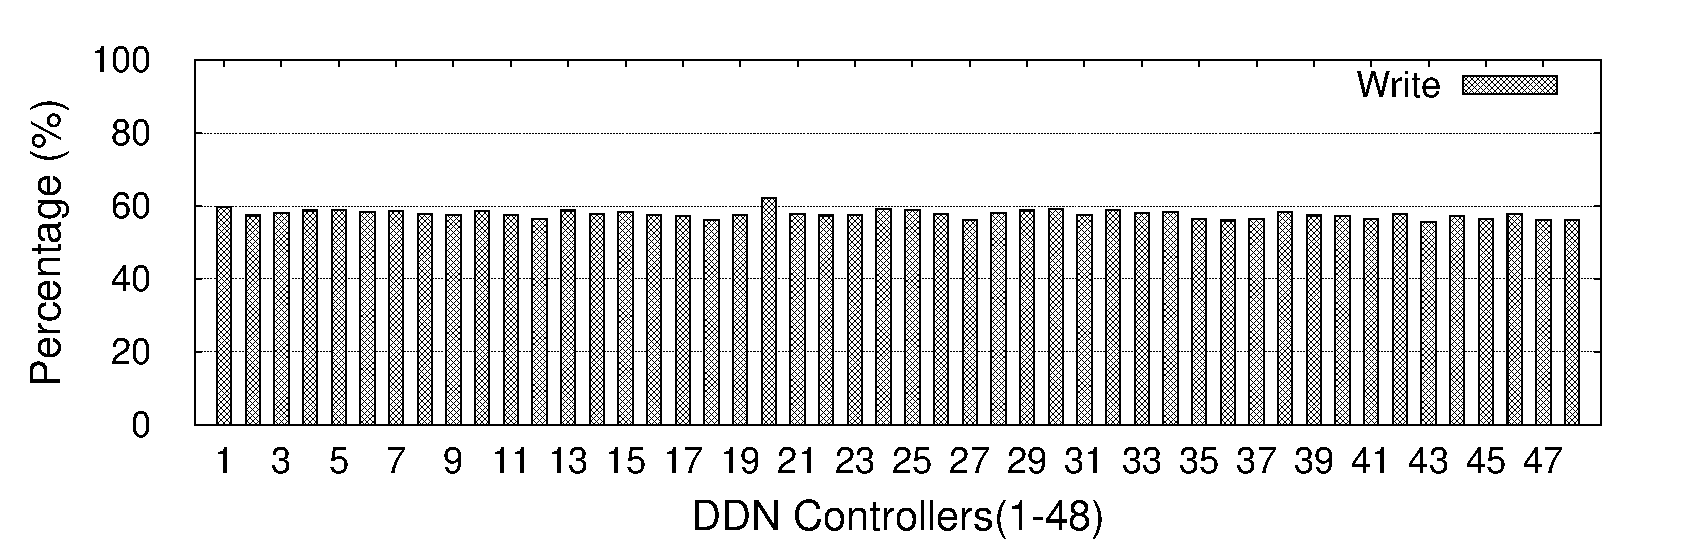
\includegraphics[width=0.5\textwidth]{./figs/spider1-wr-ratio.eps}}\\
{(a) Spider 1}\\
{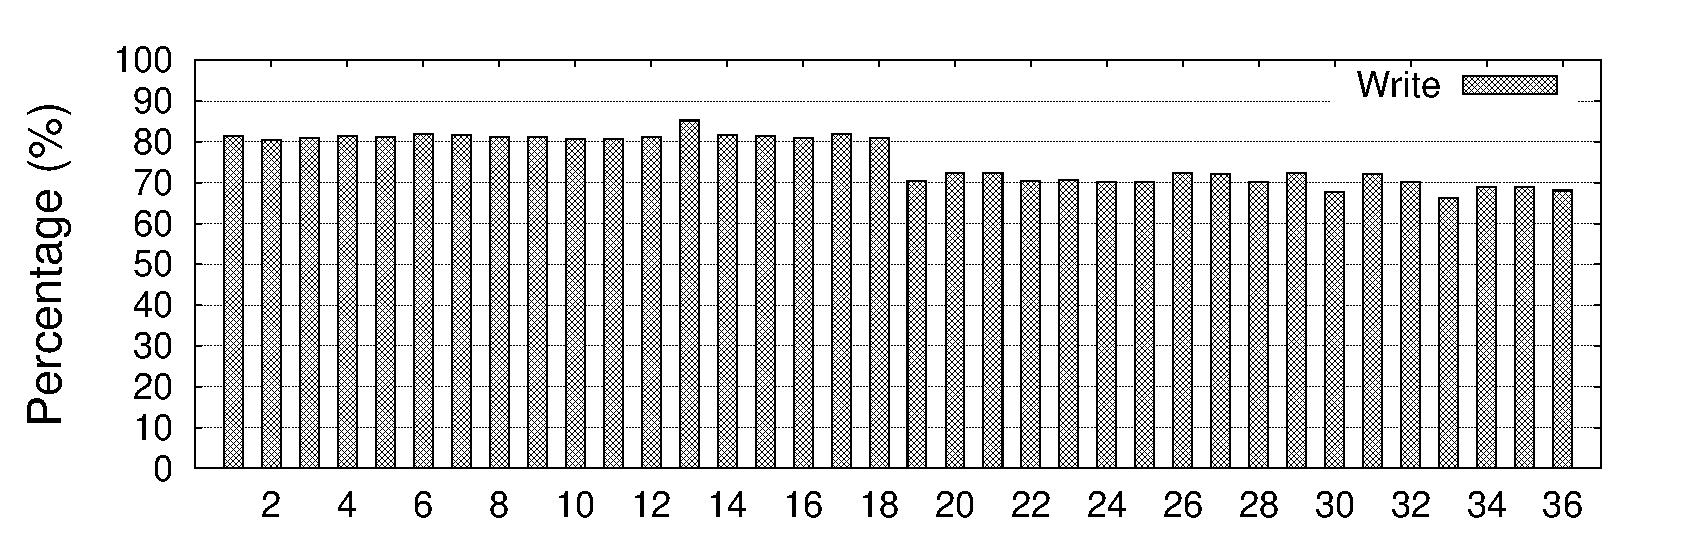
\includegraphics[width=0.5\textwidth]{./figs/spider2-wr-ratio.eps}}\\
{(b) Spider 2}\\
\end{tabular}
\vspace{-0.1in}
\caption{Read vs Write on the Storage System}
\label{fig:rwratio}
\end{center}
\end{figure}

\subsubsection{Peak Bandwidth Usage}

Figures~\ref{fig:ddnpeakBW}(a) and ~\ref{fig:ddnpeakBW}(b) show the
peak read and write bandwidth observed at the DDN RAID controllers for Spider 1
and Spider 2, respectively.  Figure~\ref{fig:ddnpeakBW}(b) shows that the peak read
bandwidth observed was 90\% of the 
maximum theoretical performance for Spider 1 (3 GB/s per controller); we observed 80\% of the maximum bandwidth for 
Spider 2 (36 GB/s per controller). For writes, the bandwidth observed was 50\% for Spider 1 and 70\% for
Spider 2. These values show us that our current read I/O workloads are achieving a 
slightly lower peak value of the overall percentage. The good news is that the write
operations on Spider 2 are obtaining a higher percentage of the peak performance.
This can be
attributed to better formed write I/O being issued from the Titan supercomputer. While 
the exact reasons for this are under the investigation, we believe the middleware 
libraries such as ADIOS~\cite{adios} are helping to improve the I/O characteristics. 


\begin{figure}[!thb]
\begin{center}
\begin{tabular}{c}
%\hspace*{-1cm}                                                           
{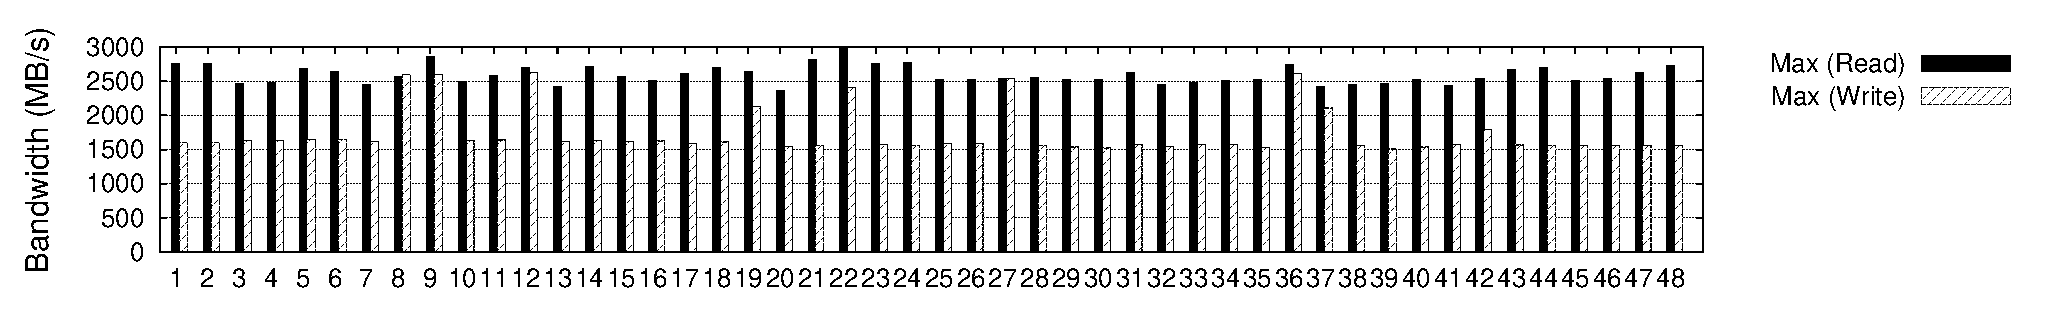
\includegraphics[width=0.450\textwidth]{./figs/spider1-bw-perc-max.eps}}\\
{(a) Spider 1}\\
\\
{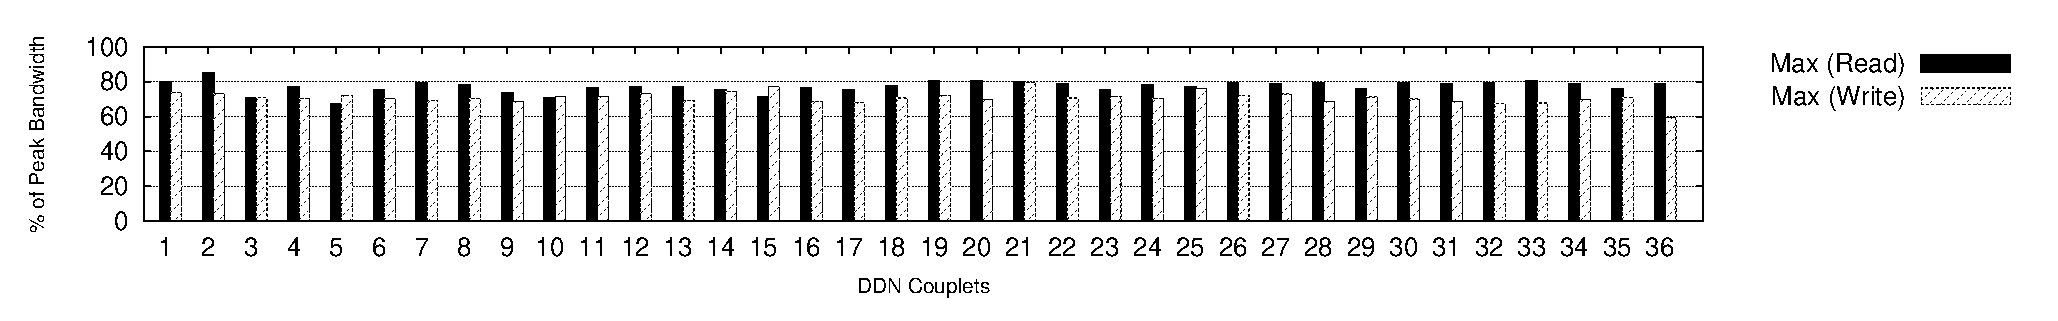
\includegraphics[width=0.450\textwidth]{./figs/spider2-bw-perc-max.eps}}\\
{(b) Spider 2}\\
\end{tabular}
\vspace{-0.1in}
\caption{Peak bandwidth usage at the RAID controllers}
\label{fig:ddnpeakBW}
\end{center}
\end{figure}

\subsubsection{Spider 2 Usage Stats}

Figure~\ref{fig:bwUsage}, shows the aggregate bandwidth (i.e. the sum of read
and write bandwidth) observed on Spider 2. We do not have a comparable data set
for Spider 1, however, we think it is useful to share the Spider 2 data. 

The Spider 2 file system was designed to deliver greater than 1 TB/s at the file system level 
if exercised with well-formed, large, sequential I/O on a quiet system. However, under
normal production workloads, the file system is exercised by random mixed I/O
workloads. Our earlier tests showed that a single NL-SAS disk drive can achieve
20-25\% of its peak performance under random I/O workloads (with 1 MB I/O block
sizes). Extrapolating from that point, the expected Spider 2 performace should be 
at most 250 GB/s under such bursty production workloads.~\cite{bestpractices}.

As can be seen from the Figure~\ref{fig:bwUsage}, more than 95\% of the 
observed bandwidth was less than 50 GB/s. Around 4\% of the time the bandwidth
was over 50 GB/s. For less than 1\% of the time the bandwidth peaked over
250 GB/s. These values are in line with the design goals of Spider 2, as
typical scientific applications are compute intensive and perform
I/O in bursts that total less than 5\% of their compute time allocations. This suggests that these 
mixed workloads could benefit from a burst buffer storage layer to absorb and align 
their I/O.

Figure~\ref{fig:storageUsage} shows the Spider 2 space utilization. As can be
seen, more than 50\% of the capacity is currently being used.  For a sustained a
bandwidth of 250 GB/s (peak random production bandwidth) for 10 minutes in a
day, 146 TBs of data will be generated. Given the 32 PB aggregate capacity of
Spider 2, this will consume all space on Spider 2 in less than a year. To
prevent this, OLCF employs a ``purge'' policy. Periodically, files with a
timestamp older than 14 days are deleted from the Spider 2 scratch file system.
This helps maintain a utilization less than 75\% on the Spider 2 system.  

\begin{figure}[!thb]
\begin{center}
\begin{tabular}{c}
{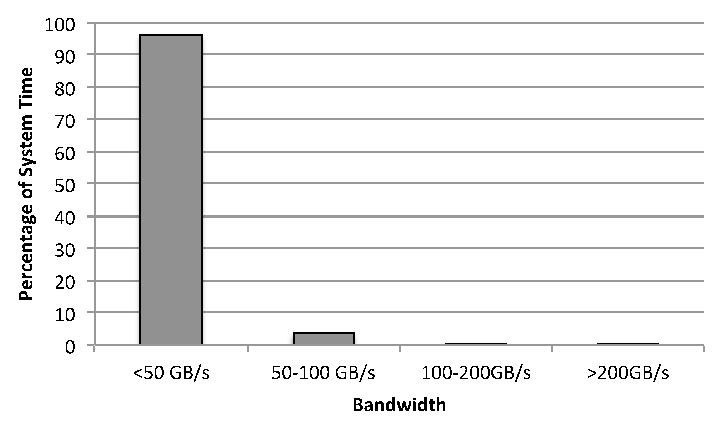
\includegraphics[width=0.40\textwidth]{./figs/bwUsage.eps}}\\
\end{tabular}
\vspace{-0.1in}
\caption{Spider 2 usage with respect to bandwidth}
\label{fig:bwUsage}
\end{center}
\end{figure}



\begin{figure}[!thb]
\begin{center}
\begin{tabular}{c}
{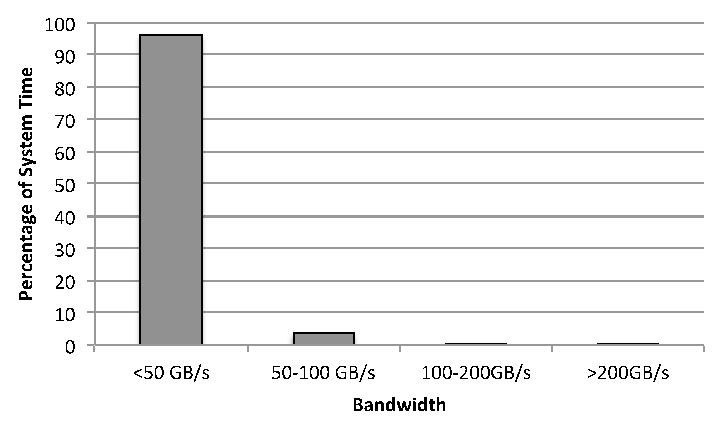
\includegraphics[width=0.40\textwidth]{./figs/storageUsage.eps}}\\
\end{tabular}
\vspace{-0.1in}
\caption{Spider 2 usage with respect to storage space}
\label{fig:storageUsage}
\end{center}
\end{figure}


\subsection{I/O Requests}
\subsubsection{Request Size distribution}



\begin{figure}[!t]
\begin{center}
\begin{tabular}{cc}
\hspace*{-1cm}                                                           
{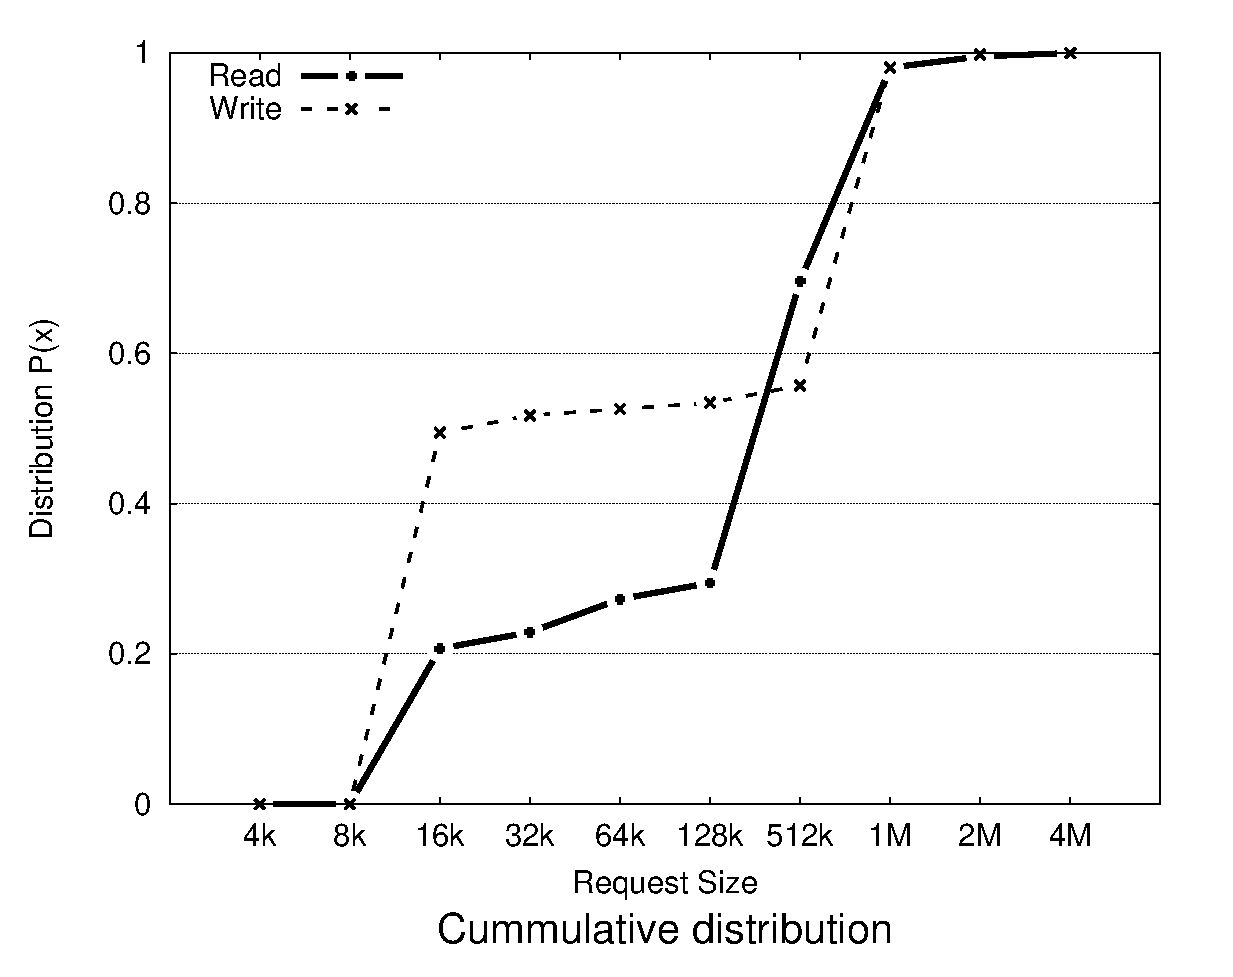
\includegraphics[width=0.27\textwidth]{./figs/spider1-reqSizeCDF.eps}}&
\hspace{-2mm}
{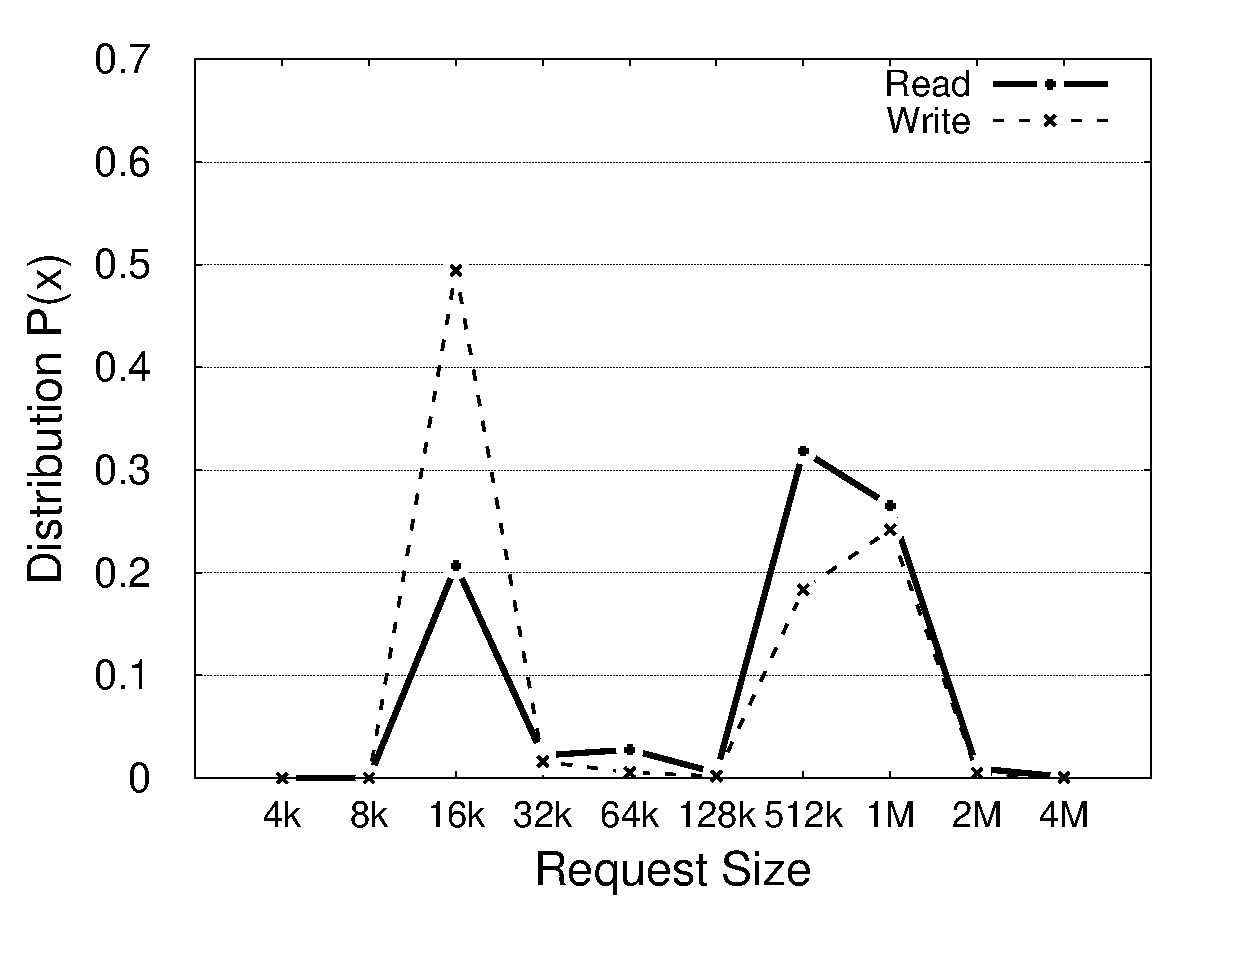
\includegraphics[width=0.27\textwidth]{./figs/spider1-reqSizePDF.eps}}\\
\small (a) CDF & \small(b) PDF \\
\end{tabular}
\vspace{-0.1in}
\captionsetup{justification=centering}
\caption{Spider 1 - Distribution of Request Sizes}
\label{fig:spider1-reqsizedist}
\end{center}
\end{figure}

\begin{figure}[!t]
\begin{center}
\begin{tabular}{cc}
\hspace*{-1cm}                                                           
{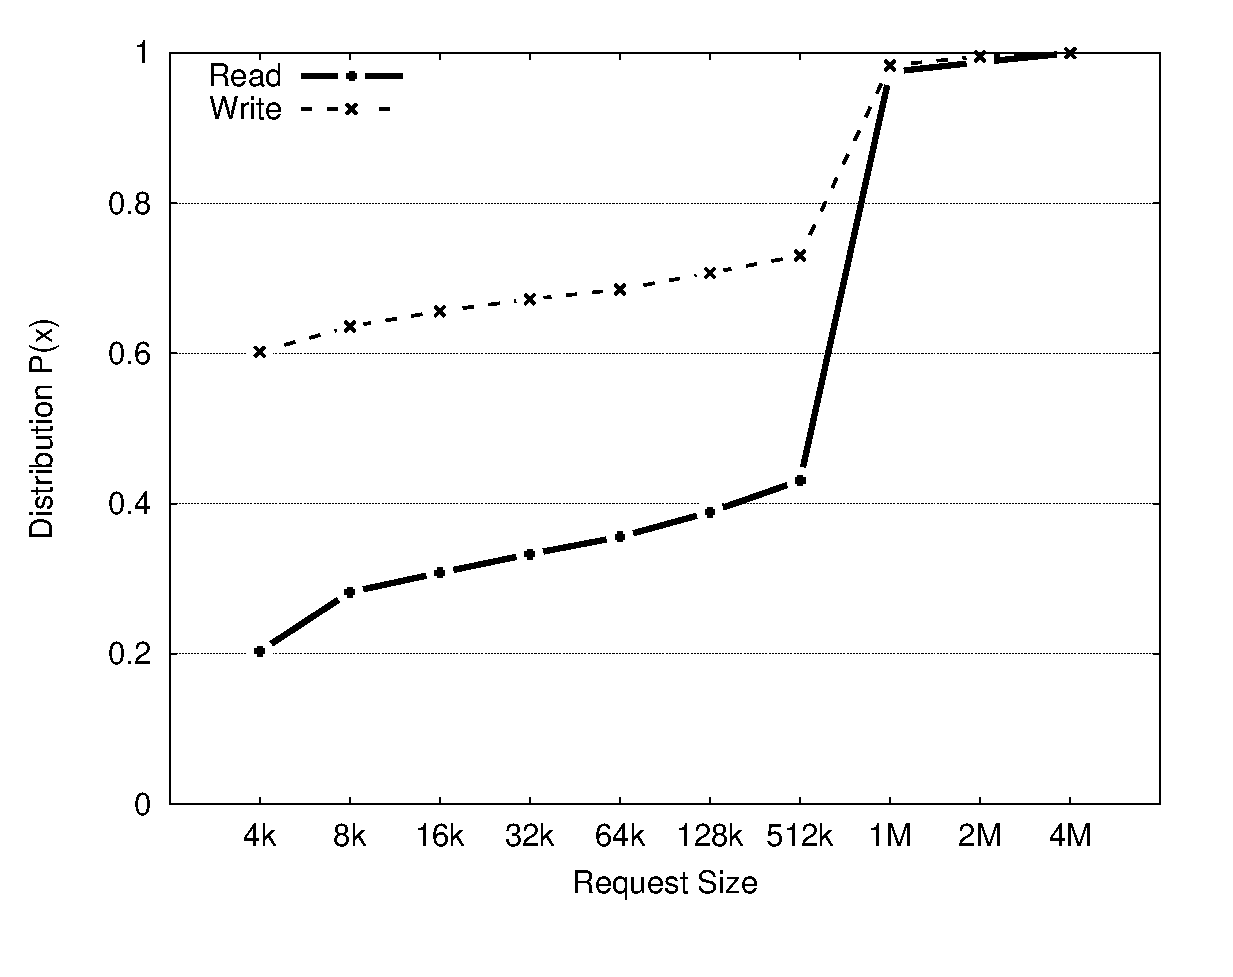
\includegraphics[width=0.27\textwidth]{./figs/spider2-reqSizeCDF.eps}}&
\hspace{-2mm}
{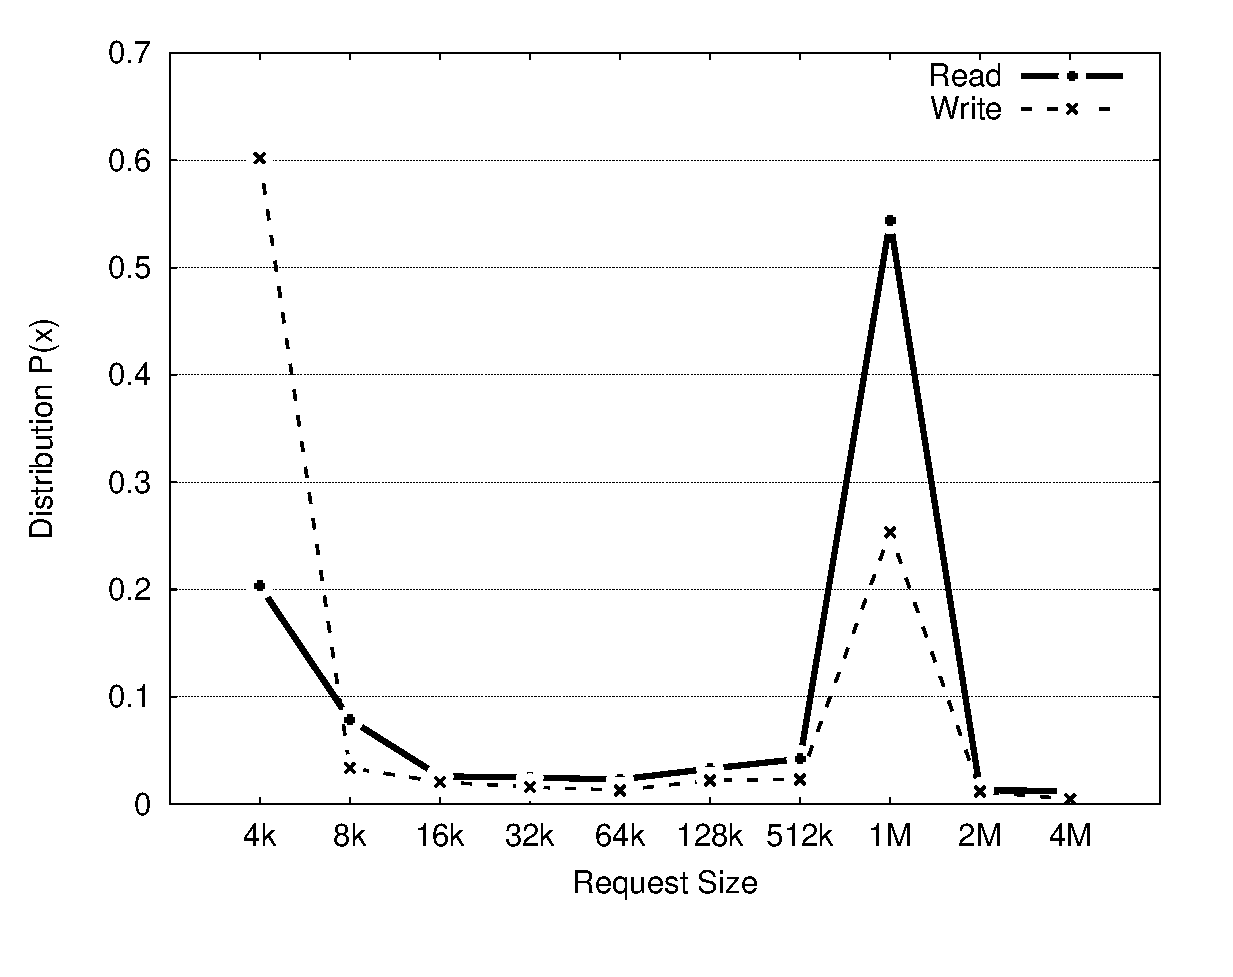
\includegraphics[width=0.27\textwidth]{./figs/spider2-reqSizePDF.eps}}\\
\small (a) CDF & \small(b) PDF \\
\end{tabular}
\vspace{-0.1in}
\caption{Spider 2 - Distribution of Request Sizes}
\label{fig:spider2-reqsizedist}
\end{center}
\end{figure}

Figures~\ref{fig:spider1-reqsizedist} and \ref{fig:spider2-reqsizedist}
show the distribution of read and write requests on Spider 1 and Spider 2,
respectively. As can be seen, there are differences. The Lustre file system
supports a range of request block sizes, the smallest being 4 kilobytes (kB)
and the largest being 4 Megabytes (MB).  However, on Spider 1, the smallest
block size we were able to monitor was 16KB, a limitation of the DDN RAID
controller. Interpreting from the CDF and PDF plots here are some interesting
observations:

\begin{itemize}

\item  60\% of write requests on Spider 2 are 4kB or less.  In Spider 1, we were
unable to distinguish between the 4kB, 8kB and 16kB sizes, which accounted for 50\%
of the write requests. Accounting for this and comparing Spider 1 and 2 file
size distributions, it can be seen that there are 10\% more small block
requests (i.e.  smaller than 8kB) on Spider 2 for write operations. Please
remember that these are directly obtained from the DDN controllers not from the
file system. One possible explanation for this increase could be an increase in the local
file system (ldiskfs) metadata operations. Another possible explanation could be an
increase in the number of controller-level background disk integrity check 
(i.e. scrubbing) events.
The exact cause of this increase is unknown at this point and it is being
investigated.  For read operations, Spider 1 and Spider 2 behave the same for
small files; the distribution has not changed.

\item  For writes, 70\% of the requests on Spider 2 are less than or
equal to 512kB, whereas on Spider 1 only 55\% of the requests were less than
or equal to 512kB. It is worth noting that the data presented in this paper are
 gathered in
different years, the application versions have changed, and there was a
different mix of applications running as the data were collected. The OLCF
traditionally has a large mix of applications that have well-formed I/O or are
using middleware libraries such as ADIOS \cite{adios}. The latest round of
applications do not have this robustness in their I/O patterns, and have shown
to have some pathological tendencies. These smaller files and request sizes
that are more focused on read operations are large performance drains on a
system that was designed to perform 1MB sequential write and read I/O
operations. 

\item On Spider 2 over 50\% of reads were 1MB, similar to Spider 1 combined
512kB and 1MB were 50\%. However, only 25\% of writes on Spider 2 are 1MB,
whereas on Spider 1 over 45\% of writes where either 512kB or 1MB. We postulate
again that the Application workload of the OLCF is different enough at the
times of measurement to show this difference in the distribution.

\item   On Spider 1, we observed a large number of 512kB requests for both read
and write requests. This was due to problems in the {\tt dm-multipath} \cite
{mpath}
package that was available for the version of the Linux operating system that
was employed. This version had a bug that broke up a 1024kB I/O request into 2
512kB requests. Later versions addressed this performance problem by not
breaking up the I/O request. Additionally Spider 1 used the {\tt deadline} I/O
request scheduler which allowed the kernel to re-order some I/O
requests.  In 2011, Spider 1 was moved to the  {\tt noop} scheduler, and this
phenomenon disappeared. We see the same drop in 512kB requests for Spider 2 as
well. Finally, changes to the {\tt ib\_srp} kernel module allow more queued
requests
and better memory handling of a larger queue through scatter\/gather tables.
This allowed fully queuing 1024kB requests and pushing them all the way to the
DDN controller. As a result of these 3 changes the number of 512kB requests
have been dramatically reduced for Spider 2.  \end{itemize}

\subsubsection{Request Size Latency distribution}

With the new DDN SFA API, now we have the capability of collecting I/O request
service latencies. Figure~\ref{fig:spider1-reqLat} shows Spider 2 request
service latency distributions. Service latency here includes the total sum of
the time spent on the queue and the time spent on fetching/putting data from/to
the disk. As can be seen from the figure, 90\% of reads and more than 80\%
write requests are serviced at most in 16ms and this is the finest granularity
the DDN API can provide. 

The SFA12KX's software incorporates newer caching algorithms that are designed
to lower the latency for certain operations, and with the readahead cache
disabled and ReACT\textsuperscript{TM} enabled, we see this highly desirable
distribution of latencies of 16ms or less.

\begin{itemize}

\item The SFA12KX disk controller has the ability to analyze incoming I/O
request stream and begin to aggressively read-ahead on the disk to internal
cache. The hope is that a large read can be sped up by hiding the latency of
the seek if the data is in cache.  In our experience and testing, this was a
very large hindrance to performance in workloads that mimic the many file read
operations from Titan's compute nodes. This is due to the algorithm caching the
wrong data, having to invalidate the cache, seek to the location on disk, cache
that data, and then repeat with the next read request. By disabling the
read-ahead cache, we dramatically lower the latency of the non-sequential read
requests we see in the production environment. 

\item The Real-time Adaptive Cache Technology
(ReACT\textsuperscript{TM})\cite{ReACT} feature was developed to make the SFA
platforms more attractive from an IOPS perspective. The feature's main goal is
to speed up the performance of the large 1MB write requests, avoiding caching
the I/O on the partner controller. The decision to only cache <1MB write
operations relieves a bottleneck that earlier versions of DDN's products did
poorly - including the S2A 9900's that Spider 1 was constructed of. In earlier
versions of the product you could either mirror your cache on the partner
controller for data resilience in the face of controller failure, or you could
disable the cache and get performance for the large streaming 1MB (or larger)
writes. ReACT gives a framework where the best of both worlds can exist.  A 1MB
write can be written directly to disk, which is the lowest latency possible for
that operation. A 4kB can be written into controller cache and also mirrored to
the partner controller in about the same amount of time, which is far faster
than committing that operation to the disk. We feel that this feature has
allowed Spider 2 to reach the low latencies across the spectrum of write
request sizes and is a large benefit to our users. 

\end{itemize}


  

\begin{figure}[!t]
\begin{center}
\begin{tabular}{cc}
\hspace*{-1cm}                                                           
{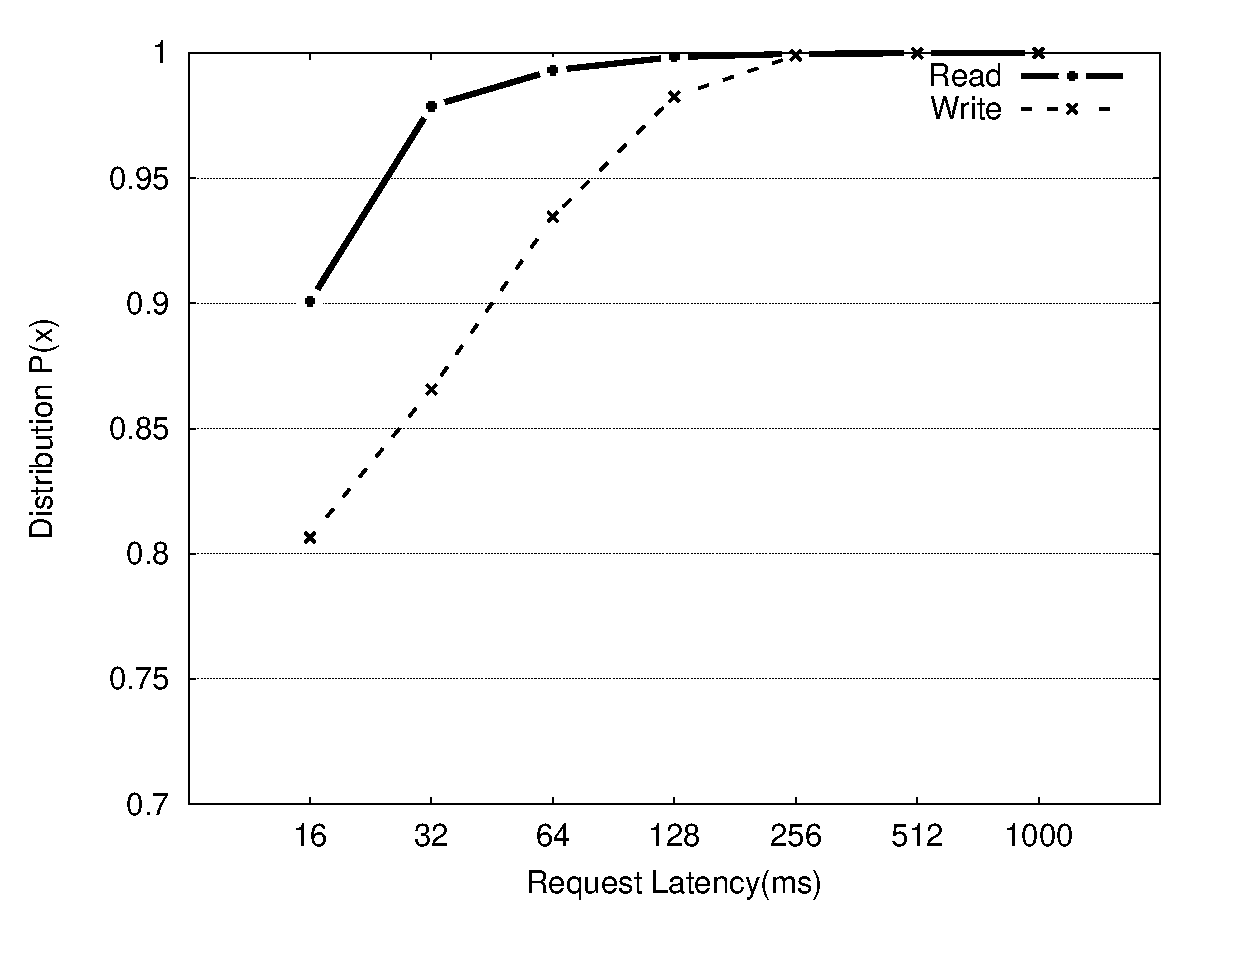
\includegraphics[width=0.27\textwidth]{./figs/spider2-reqLatCDF.eps}}&
\hspace{-2mm}
{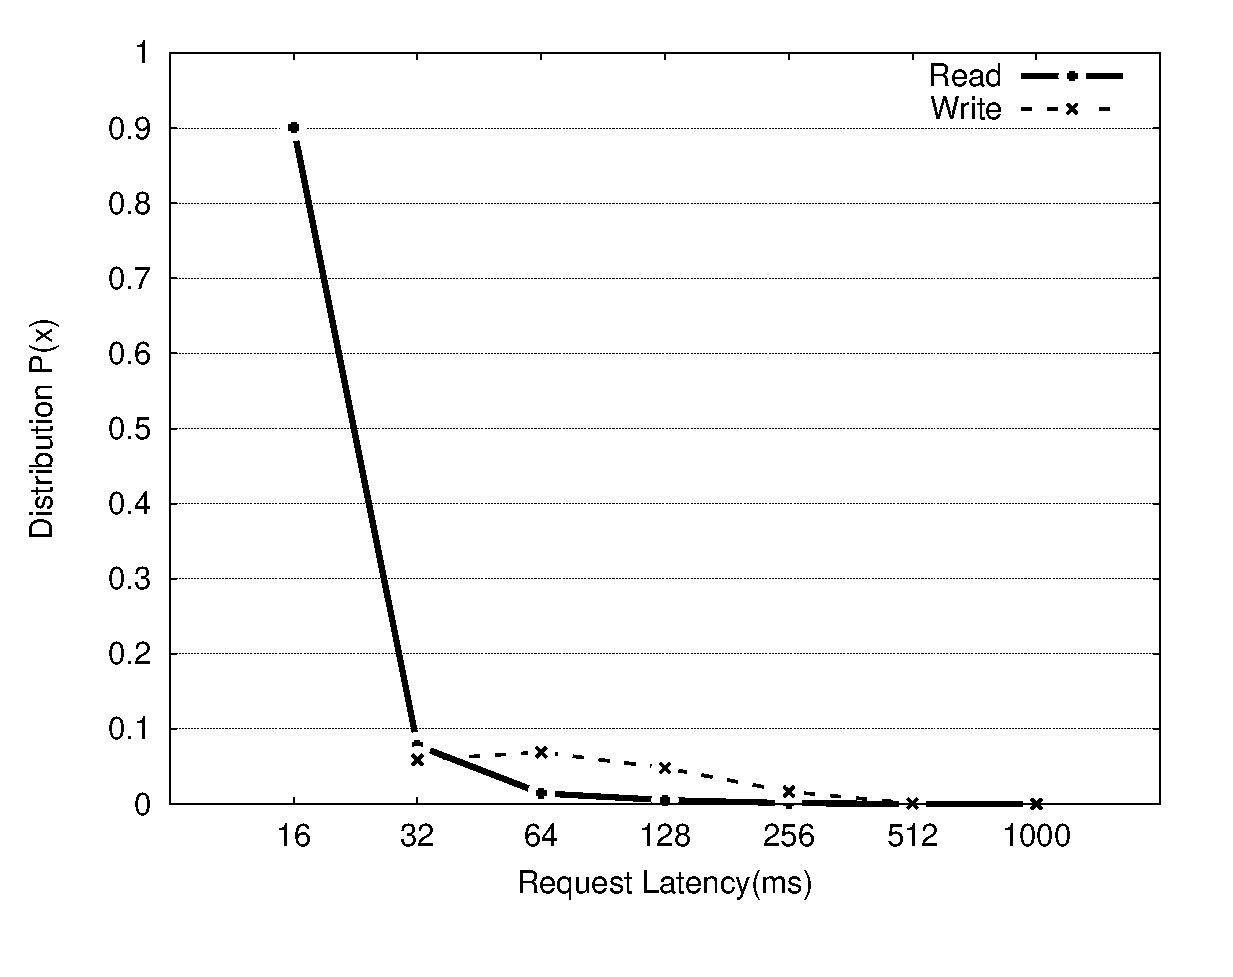
\includegraphics[width=0.27\textwidth]{./figs/spider2-reqLatPDF.eps}}\\
\small (a) CDF & \small(b) PDF \\
\end{tabular}
\vspace{-0.1in}
\caption{Spider 2 - Distribution of Request Service Time(latency)}
\label{fig:spider1-reqLat} 
\end{center}
\end{figure}
